% Exemple pour insérer de bonnes figures dans un article en format 2 colonnes, sans devoir redimensionner (utiliser un facteur d'échelle de 1 dans LaTeX lors de l'insertion des figures)

% Example for inserting good figures in an article in two-columns format, without having to resize (use a scale factor of 1 in LaTeX when inserting figures)

\documentclass{standalone}

% Ne pas trop toucher au préambule, ça marche bien!
%
% Do not touch the preamble too much, it works well!

% Il est cependant toujours possible d'ajouter des "packages" au besoin.
% If need be, you can include other packages.
\usepackage{pgfplots} % Include package for TikZ and PGF plot
\usepackage{anyfontsize} % Permet de modifier manuellement la taille de la police / Enables changing the font size manually 
\tikzset{>=latex}
\usetikzlibrary{arrows.meta}

% Véritable début du code pour la figure
% Actual beginning of the code for the figure
\begin{document}

% Le facteur d'échelle (scale=x) permet de changer la taille du texte au complet dans la figure.
% The scale factor (scale=x) allows changing the size of the entire text in the figure.
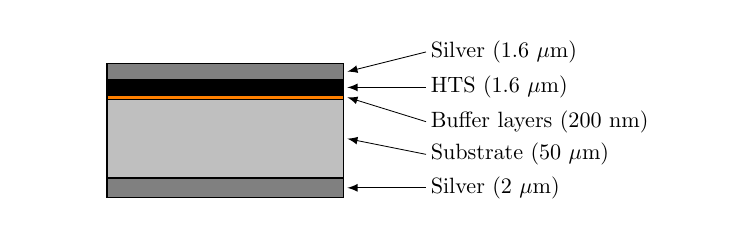
\begin{tikzpicture}[every node/.style={scale=0.8}]

% Commentaire: par défaut, la largeur des lignes est de 0.4pt, ce qui représente environ 0.14 mm (1 pt = 0.0135" = 0.3429 mm). Les dimensions sont par défaut en cm.
% La largeur d'une colonne dans un article est d'environ 8.5 cm.
% Il faut essayer de composer les figures avec ces échelles.

% The width of a column in an article is about 8.5 cm.
% You should try to create the figures with these dimensions.
%
% Pour une liste des couleurs prédéfinies, voir cette page :  / For a list of predefined colors, consult: https://en.wikibooks.org/wiki/LaTeX/Colors

% Juste pour définir la zone de dessin et fixer les dimensions absolues de la figure.
% Just to define the drawing area and set the absolute dimensions of the figure.

% C'est plus facile de modifier l'origine de cette figure que de déplacer par la suite toutes les coordonnées du dessin au complet.
% It is easier to change the origin of this figure than to move all the coordinates of the entire drawing afterwards.

% Il y a aussi moyen de dessiner en coordonnées relatives, mais mais ce n'est pas le cas ici.
% There is also a way to draw using relative coordinates, but it is not the case here.
\draw [draw=white, line width=0.5pt] (0.0,0.8) rectangle ++(8.75,2.35);

% Début de la figure proprement dite
% Beginning of the actual figure
\filldraw [draw=black, line width=0.5pt, fill=gray] (1,1) rectangle ++(3,0.25);
\filldraw [draw=black, line width=0.5pt, fill=lightgray] (1,1.25) rectangle ++(3,1);
\filldraw [draw=black, line width=0.5pt, fill=orange] (1,2.25) rectangle ++(3,0.05);
\filldraw [draw=black, line width=0.5pt, fill=black] (1,2.30) rectangle ++(3,0.2);
\filldraw [draw=black, line width=0.5pt, fill=gray] (1,2.50) rectangle ++(3,0.2);

% Flèches et étiquettes
% Arrows and labels
\draw[<-,black,line width=0.3pt] (4.05,2.6) -- ++(1,0.25) node[right, inner sep=2] {Silver (1.6~$\mu$m)};
\draw[<-,black,line width=0.3pt] (4.05,2.4) -- ++(1,0) node[right, inner sep=2] {HTS (1.6~$\mu$m)};
\draw[<-,black,line width=0.3pt] (4.05,2.275) -- ++(1,-0.31) node[right, inner sep=2] {Buffer layers (200~nm)};
\draw[<-,black,line width=0.3pt] (4.05,1.75) -- ++(1,-0.2) node[right, inner sep=2] {Substrate (50~$\mu$m)};
\draw[<-,black,line width=0.3pt] (4.05,1.125) -- ++(1,0) node[right, inner sep=2] {Silver (2~$\mu$m)};

%\draw[->,>=stealth,-biggertip,black] (5,1.0,10) -- (5,2,10);	
					
\end{tikzpicture}

\end{document}
